\documentclass[lettersize,journal]{IEEEtran}
\usepackage{amsmath,amsfonts}
\usepackage{algorithmic}
\usepackage{array}
\ifCLASSOPTIONcompsoc
    \usepackage[caption=false, font=normalsize, labelfont=sf, textfont=sf]{subfig}
\else
\usepackage[caption=false, font=footnotesize]{subfig}
\fi
\usepackage{textcomp}
\usepackage{stfloats}
\usepackage{url}
\usepackage{verbatim}
\usepackage[extract=python]{memoize}
% -- ADDED PACKAGES  after memoize --
\usepackage{graphicx}
\usepackage{circuitikz}
\usepackage{tikz}
\usepackage{algorithm}
\usepackage{pgfplots}
\usepackage{booktabs}
\usepackage{makecell}

% \usepackage{algpseudocode}


% \pgfplotsset{compat=1.18} % Set the compatibility level for pg
\usetikzlibrary{shapes.geometric, arrows, positioning, fit, backgrounds}



\definecolor{ieeeblue}{RGB}{0,118,186}      % IEEE Blue
\definecolor{ieeered}{RGB}{214,39,40}       % IEEE Red  
\definecolor{ieeegreen}{RGB}{23,156,82}     % IEEE Green



\newcommand{\der}{{\rm d}}
\newcommand{\R}{\mathcal{R}}
\newcommand{\C}{\mathcal{C}}
\newcommand{\M}{\mathcal{M}}
\newcommand{\G}{\mathcal{G}}
\newcommand{\Ron}{R_{\rm ON}}
\newcommand{\Roff}{R_{\rm OFF}}
\newcommand{\von}{V_{\rm ON}}
\newcommand{\voff}{V_{\rm OFF}}
\newcommand{\q}{q}
\newcommand{\ua}{v}
\newcommand{\ia}{i}
\newcommand{\phia}{\varphi}
\newcommand{\xw}{x}
\newcommand{\dert}[1]{\frac{{\rm d} {#1}}{{\rm d} t} }
\newcommand{\inv}[1]{\frac{1}{#1} }
\newcommand{\equal}{=}



\usepackage[
  backend=biber,
  style=ieee,
  minnames=1,
  maxcitenames=2, maxbibnames=6
]{biblatex}

\addbibresource{bibliography.bib}


\newcommand{\TODO}[1]{\textcolor{red}{#1}}

\hyphenation{op-tical net-works semi-conduc-tor IEEE-Xplore}
\def\BibTeX{{\rm B\kern-.05em{\sc i\kern-.025em b}\kern-.08em
    T\kern-.1667em\lower.7ex\hbox{E}\kern-.125emX}}
\usepackage{balance}
\begin{document}
\title{How to Use the IEEEtran \LaTeX \ Templates}
\author{IEEE Publication Technology Department
  \thanks{Manuscript created October, 2020; This work was developed by the IEEE Publication Technology Department. This work is distributed under the \LaTeX \ Project Public License (LPPL) ( http://www.latex-project.org/ ) version 1.3. A copy of the LPPL, version 1.3, is included in the base \LaTeX \ documentation of all distributions of \LaTeX \ released 2003/12/01 or later. The opinions expressed here are entirely that of the author. No warranty is expressed or implied. User assumes all risk.}}

\markboth{Journal of \LaTeX\ Class Files,~Vol.~18, No.~9, September~2020}%
{How to Use the IEEEtran \LaTeX \ Templates}

\maketitle

\begin{abstract}
  This document describes the most common article elements and how to use the IEEEtran class with \LaTeX \ to produce files that are suitable for submission to the Institute of Electrical and Electronics Engineers (IEEE).  IEEEtran can produce conference, journal and technical note (correspondence) papers with a suitable choice of class options.
\end{abstract}

\begin{IEEEkeywords}
  Class, IEEEtran, \LaTeX, paper, style, template, typesetting.
\end{IEEEkeywords}


\section{Introduction}
\IEEEPARstart{N}{umerous} memristor models have been proposed in the scientific literature following the discovery of memristive behavior at the nanoscale. The original model, introduced in~\cite{Strukov2008}, conceptualizes the memristor as a series connection of two variable resistances corresponding to the conductive and insulating regions of the thin film. To more accurately model Self-Directed Channel (SDC) memristors, M.~Nugent and T.~Molter proposed the generalized \textit{Mean Metastable Switch} (MMS) model, which is a semi-empirical formulation. In this approach, the time derivative of the internal state variable is defined as a function of both the transition probabilities between metastable states and the current value of the state variable~\cite{Molter2016}. In~\cite{Lee2024}, the authors attempted to model memristive behavior using the \textit{Physics-Informed Neural Networks} (PINNs) framework. Although the reported results indicate the potential of this method, the study is not grounded in experimental measurements of physical memristor devices. Instead, the analysis is limited to comparisons with the outcomes of existing simulation models. Moreover, the training data employed during the neural network learning process were generated based on previously developed theoretical models, thereby limiting the ability to assess the method's accuracy in the context of real-world physical systems.


In~\cite{Ricky2018}, the authors introduce the concept of deep neural models in which the dynamics of the hidden state are governed by an \textit{ordinary differential equation} (ODE). The training process is performed in an end-to-end manner, meaning that all parameters are optimized simultaneously within a single training routine. A key innovation of the proposed approach is a novel backpropagation technique, which relies on solving the corresponding adjoint ODE backward in time using \textit{adjoint sensitivity methods}. This formulation enables efficient gradient computation and facilitates the application of neural ODEs in various architectures, including continuous-depth residual networks and generative flow-based models.


In~\cite{Ricky2021}, the authors extend the classical Neural ODE framework to enable the modeling of discontinuous events in continuous time—without requiring prior knowledge of the number or timing of such events. The proposed differentiable event functions allow for efficient simulation of hybrid systems, such as systems with collisions, state-switching mechanisms, or point processes. This development opens up new possibilities for modeling and training systems with discrete control inputs and non-smooth dynamics.


The present study aims to investigate the feasibility of modeling Self-Directed Channel (SDC) memristors using artificial neural networks, and to compare the effectiveness of this approach with that of existing theoretical models. Specifically, we focus on the application of Neural Ordinary Differential Equation (Neural ODE) models to simulate the behavior of SDC memristors, utilizing experimental data obtained from real physical systems.

Our objective is to assess whether neural network-based models can accurately reproduce the dynamic characteristics of SDC memristors, and to determine whether they offer any advantages over traditional theoretical approaches—particularly in terms of modeling flexibility, accuracy, and applicability to real-world, measurement-driven scenarios.


\section{Materials and Methods}
\noindent This study utilizes experimental data obtained from physical Self-Directed Channel (SDC) memristors doped with tungsten. The structure and properties of these devices have been described in detail in the literature, e.g., in~\cite{Garda2024, Campbell2017}.

The experimental setup, illustrated in Fig.~\ref{fig:memristor_setup}, consisted of an SDC memristor connected in series with a resistor. The sinusoidal input voltage was supplied by an arbitrary waveform generator, while the voltage signals were measured using a data acquisition (DAQ) system.

Measurements were carried out for various combinations of supply voltage amplitudes and frequencies. Specifically, the amplitude of the applied voltage was varied as \(V_s \in \{0.5,\ 1.0,\ 1.5\}~\mathrm{[V]}\), and the frequency was selected from the set \(f \in \{1,\ 5,\ 10,\ 20,\ 50,\ 100\}~\mathrm{[Hz]}\).

\begin{figure}[!t]
  \centering
  \resizebox{2.5in}{!}{
\begin{circuitikz}[american, cute inductors, transform shape]
  \draw (0, 0)
  to [vsourcesin, fill=blue, l=\(v_s \equal V_s\sin (2 \pi f_s \cdot t)\)] (1,0)
  to  [memristor, fill=yellow, l=\(M\), v=\(v_{m}\), invert] (4,0)
  to [short, i=\(i_{m}\)] (4.5,0)
  to [R, l=\(R_s\), v=\(v_{r}\)] (6.5,0);
  \draw (0,0) -- (-0.5,0) node[rground]{};
  \draw (6.5,0) -- (7,0) node[rground]{};
  \draw (0,-2.5);
\end{circuitikz}}
  \vspace{-0.5in}
  \caption{Schematic diagram of the measurement setup used for the SDC memristor. The device is connected in series with a resistor, and the input voltage is applied via an arbitrary waveform generator. Voltage measurements are acquired using a data acquisition (DAQ) system.}
  \label{fig:memristor_setup}
\end{figure}

\subsection{Modeling with Neural Networks}
\noindent The analyzed model is grounded in the general theoretical framework of memristive devices, originally introduced in~\cite{Chua1976}, and is expressed through equations~\eqref{eq:memristor_model1}.
\newcommand{\xvec}{\mathbf{x}}
\begin{align}
  \begin{split}
    \label{eq:memristor_model1}
    \ua(t)                    & = \M \big(\xvec(t),\ua(t)\big) \, \ia(t), \\
    \frac{\der \xvec}{\der t} & = f\big(\xvec(t),\ua(t)\big)
  \end{split}
\end{align}
where \(\xvec\) denotes the vector of internal state variables, whose temporal evolution is governed by the dynamic function \(f\), and \(\M\) represents the memristance of the device. A fundamental challenge in memristor modeling lies in accurately identifying the functional forms of \(\M(\xvec,\ua)\) and \(f(\xvec,\ua)\).

In this study, two neural network–based modeling approaches are investigated. The first, denoted as \textbf{Det-MemODE}, employs a deterministic formulation of the memristor conductance. The second, referred to as \textbf{Dual-NN-MemODE}, adopts a data-driven strategy in which the conductance is directly modeled using neural networks. Although both approaches utilize neural networks to approximate the dynamic function \(f(\xvec(t), \ua(t))\), they differ fundamentally in the representation of the memristor conductance.

In the first approach (Det-MemODE), the memristor conductance is defined on the basis of the physical mechanisms underlying self-directed channel (SDC) devices. In such memristors, the resistance evolves as a result of \(\mathrm{Ag^+}\) ion migration and the dynamic formation of conductive filaments. Consequently, the device conductance exhibits a continuous transition between distinct resistance states. This transition can be described as a weighted combination of the limiting resistance values, modulated by the internal state variable. Formally, the memristor conductance is expressed as \(G_m(x) = \M(x)^{-1}\), where \(\M(x)\) denotes the state-dependent resistance.
\begin{equation}
  G_{m}(x) = \frac{x}{R_{\rm ON}} + \frac{1 - x}{R_{\rm OFF}},
  \label{eq:conductance}
\end{equation}
where \(\Ron\) and \(\Roff\) denote the resistances in the low-conductance and high-conductance states, respectively. For all of these approaches also the function \(f(\xvec(t), \ua(t))\) was implemented using an artificial neural network, whose conceptual architecture is illustrated in Fig.~\ref{fig:nn_structure} for the Det-MemODE and in Fig.~\ref{fig:nn_structure_dual} for the Dual-NN-MemODE.

\begin{figure}[t!]
  \centering
  \includegraphics[width=\columnwidth]{figs/Rysowanie_schematów (2).pdf}
  \caption{ Conceptual diagram illustrating the use of a neural network to simulate the dynamics of the memristor, for the Det-MemODE, with schematic representation of the Neural ODE framework, where an artificial neural network (ANN) computes the derivative function \(f_x(x,v)\), which is then integrated by an ODE solver to predict the state at the next time step \(x(t + \Delta t)\). The dashed feedback loop indicates the recurrent nature of the process, where the output state is fed back as input for subsequent predictions.}
  \label{fig:nn_structure}
\end{figure}

\begin{figure}[t!]
  \centering
  \includegraphics[width=\columnwidth]{figs/Rysowanie_schematów (3).pdf}
  \caption{ Conceptual diagram illustrating the use of a neural network to simulate the dynamics of the memristor, for the Dual-NN-MemODE, with schematic representation of the Neural ODE framework, where an artificial neural network (ANN) computes the derivative function \(f_x(x,v)\), which is then integrated by an ODE solver to predict the state at the next time step \(x(t + \Delta t)\). The dashed feedback loop indicates the recurrent nature of the process, where the output state is fed back as input for subsequent predictions.}
  \label{fig:nn_structure_dual}
\end{figure}

The neural network consists of interconnected nodes (neurons) that process information through weighted connections. Each neuron in the network computes its output according to:

\begin{equation}
  y = \sigma\left(\sum_{i=1}^{n} w_i x_i + b\right)
\end{equation}

where \(w_i\) are the weights that determine the strength and importance of each input connection \(x_i\), \(b\) is the bias term that provides an adjustable threshold for neuron activation, and \(\sigma\) is the activation function (e.g., sigmoid, ReLU, or tanh) that introduces non-linearity into the model.

The weights represent the learnable parameters that encode the relationship between inputs and outputs, while biases allow neurons to shift their activation threshold, enabling the network to better fit the training data even when all inputs are zero. During the optimization process, the network parameters (weights and biases) are tuned jointly with the values of \(R_{\rm ON}\) and \(R_{\rm OFF}\).

The learning process involves iteratively adjusting the network parameters to minimize a loss function that quantifies the difference between predicted and target outputs. This is  achieved through backpropagation algorithm combined with gradient descent optimization, where gradients of the loss function with respect to each parameter are computed and used to update the weights and biases in the direction that reduces the overall error.

\subsection{Neural Network Architecture Design}

\noindent The neural network model development and training pipeline was implemented using the \texttt{PyTorch} deep learning framework, described in~\cite{paszke2019pytorchimperativestylehighperformance}, within the \texttt{Python} programming environment, leveraging its automatic differentiation capabilities. To enable seamless integration of ordinary differential equations (ODEs) within the neural network training paradigm, the specialized \texttt{torchdiffeq} library was employed. This library provides differentiable ODE solvers that facilitate efficient gradient computation with respect to solution trajectories through the adjoint sensitivity method, well described in~\cite{Ricky2018, Ricky2021, torchdiffeq}. This approach enables end-to-end training of neural differential equation models by maintaining gradient flow through the numerical integration process, which is essential for learning dynamic systems governed by differential equations.

Specifically, the \texttt{dopri5} (Dormand-Prince 5th order) adaptive Runge-Kutta solver was utilized for its superior balance between computational efficiency and numerical accuracy. This solver employs embedded error estimation for adaptive step-size control, ensuring stable integration of the memristor dynamics while maintaining computational tractability during training.

The neural network architecture is illustrated in Figure~\ref{fig:nn-arch} and incorporates a strategically designed bottleneck configuration with dimensional two time reduction in the initial and final hidden layers. This architectural choice addresses several critical aspects of neural ODE training and memristor system modeling, like:
\begin{itemize}
  \item Dimensional reduction at the start and end of the network significantly decreases the total parameter count,
  \item  Parameter count reduction contributes to more stable optimization dynamics by limiting the search space complexity
  \item Dimensional reduction helps mitigate gradient vanishing and explosion problems that commonly arise in deep networks processing long temporal sequences
  \item  The bottleneck structure implicitly enforces a low-dimensional manifold assumption consistent with the underlying physics of memristor dynamics
\end{itemize}


\begin{figure}[ht!]
  \centering
  \resizebox{2in}{!}{%
    \begin{tikzpicture}[
    neuron/.style={circle, draw, minimum size=0.5cm},
    layer/.style={rectangle, draw, minimum width=3cm, rounded corners, align=center},
    arrow/.style={-{Stealth[scale=1.2]}, thick},
    activation/.style={rectangle, draw, minimum height=0.7cm, minimum width=2cm, rounded corners, fill=orange!30},
    node distance=1.5cm
    ]

    % Define the layers (now vertical)
    \node[layer, minimum height=1.2cm] (input) {Input Layer (2)};
    \node[layer, minimum height=1.2cm, below=of input] (h1) {Hidden Layer 1\\($\lfloor N/2 \rfloor$)};
    \node[activation, below=0.5cm of h1] (act1) {activation};
    \node[layer, minimum height=1.2cm, below=0.5cm of act1] (h2) {Hidden Layer 2..L-1\\($N$)};
    \node[activation, below=0.5cm of h2] (act2) {activation};
    \node[layer, minimum height=1.2cm, below=0.5cm of act2] (h3) {Hidden Layer L\\($\lfloor N/2 \rfloor$)};
    \node[activation, below=0.5cm of h3] (act3) {activation};
    \node[layer, minimum height=1.2cm, below=1cm of act3] (output) {Output Layer (1)};

    % Connect the layers
    \draw[arrow] (input) -- (h1);
    \draw[arrow] (h1) -- (act1);
    \draw[arrow] (act1) -- (h2);
    \draw[arrow] (h2) -- (act2);
    \draw[arrow] (act2) -- (h3);
    \draw[arrow] (h3) -- (act3);
    \draw[arrow] (act3) -- (output);

    % Add ODE block annotation
    \node[draw, dashed, rounded corners, fit={(h1) (h2) (h3) (act1) (act2) (act3)}, inner sep=0.5cm, label=right:Neural ODE Block] {};

\end{tikzpicture}
  }
  \caption{Architecture of the feedforward neural network used within the Neural ODE framework for memristor dynamics modeling. The network consists of an input layer receiving two inputs, multiple hidden layers with decreasing-increasing-decreasing neuron counts (\(\lfloor N/2 \rfloor, N, \lfloor N/2 \rfloor\)), activation functions between layers, and a single output. The Neural ODE block encompasses the core computational layers that approximate the derivative function \(f(\xw(t), \ua(t))\) in the differential equation system.}

  \label{fig:nn-arch}
\end{figure}


The network weights were optimized using several optimization techniques, including the \texttt{Adam} (Adaptive Moment Estimation) optimizer. The choice of optimizer and its parameters was guided by hyperparameter tuning conducted with the \texttt{Optuna} framework, as described in~\cite{Akiba2019}. The hyperparameter search space comprised the learning rate, weight decay, and batch size, while the optimal configuration was selected based on validation loss minimization. To enable adaptive control of the learning rate throughout training, the \texttt{ReduceLROnPlateau} scheduling strategy was employed. This performance-based scheduler dynamically adjusts the learning rate in response to plateaus in the monitored validation loss, thereby improving convergence stability. Specifically, the scheduler reduces the learning rate once the monitored loss stagnates, applies a predefined reduction factor, incorporates a patience interval before making adjustments, and enforces lower and upper bounds to prevent instability. This implementation strategy ensures robust and efficient training of neural differential equation models for memristor circuit simulation, integrating state-of-the-art deep learning practices with domain-specific techniques for dynamic system modeling.

\subsection{Deterministic Memristor Model for Comparison}
\noindent To evaluate the effectiveness of the proposed model, it was compared with the two deterministic models: the Mean Metastable Switch (MMS) model introduced in~\cite{Minati2020} and the  Generalized Mean Metastable Switch Memristor (GMMS) model described in~\cite{Molter2016, Ostrovskii2021}.

\subsubsection{Mean Metastable Switch (MMS) Model}
The Mean Metastable Switch (MMS) model is a simplified representation of memristor behavior, focusing on the average switching characteristics rather than the detailed dynamics. It captures the essential features of memristive switching by modeling the device as a two-state system, where the resistance can switch between a high-resistance state (HRS) and a low-resistance state (LRS) based on the applied voltage. This model describes the memristor dynamics using Eq.~\eqref{eq:mms}.

\begin{align}
  \label{eq:mms}
  \dert{x} & = \frac{1}{\tau} \big[ f_{\rm on}(t) (1-x) - f_{\rm off}(t) x \big]
\end{align}
where
\begin{align}
  f_{\rm on}(t)  & = \frac{1}{1+e^{-\beta (\ua(t)-\von)}} \label{eq:mms5b}      \\
  f_{\rm off}(t) & = 1 - \frac{1}{1+e^{-\beta (\ua(t)-\voff)}} \label{eq:mms5c}
\end{align}

where \(\beta= \frac{q}{kT}\) is a temperature-related parameter, \(\von\) denotes the switching voltage to the low-resistance state (LRS), \(\voff\) denotes the switching voltage to the high-resistance state (HRS), \(k\) is the Boltzmann constant, \(T\) is the absolute temperature, and \(q\) represents the elementary charge. The instantaneous conductance of the memristor is defined as in Eq.~\eqref{eq:conductance}.

\subsubsection{Generalized Mean Metastable Switch (GMMS) Model}
In~\cite{Molter2016}, the authors introduced the Generalized Mean Metastable Switch (GMMS) model, in which the memristor is represented as a parallel connection of two memristors and a Schottky diode. This formulation extends the original metastable switch concept by incorporating nonlinear current--voltage characteristics, thereby enabling a more accurate representation of memristor behavior across a wide range of operating conditions.

Nevertheless, the inclusion of additional parameters and nonlinearities increases the model's complexity and poses challenges for parameter optimization. In this framework, the evolution of the state variable is governed by Eq.~\eqref{eq:mms}, while the current--voltage relationship is described by the following set of equations:
\begin{align}
  \begin{split}
    i(t)      & = \phi i_m(v, t) + (1-\phi) i_d(v)                 \\
    i_d(v)    & = \alpha_f e^{\beta_f v} - \alpha_r e^{-\beta_r v} \\
    i_m(v, t) & = \G_m(x) v
  \end{split}
  \label{eq:gmms}
\end{align}
where \(\phi \in [0,1]\) is a parameter representing the fraction of the total current flowing through the memristor relative to the entire current through the device. The parameters \(\alpha_f\), \(\beta_f\), \(\alpha_r\), and \(\beta_r\) are positive constants characterizing the forward and reverse current behavior along the Schottky barrier.

In the case of the GMMS model, an additional challenge arises due to the Schottky effect, which introduces nonlinearity into the current–voltage characteristic. When the memristor is connected in series with a resistor, this requires solving a nonlinear equation of the form Eq. \eqref{eq:nonlinear_eq}. As a result, the system of ordinary differential equations is transformed into a differential-algebraic equation (DAE).
\begin{equation}
  \left\{
  \begin{aligned}
     & v_s(t)    = v_r(t) + v_m(t)                                                   \\
     & \dert{x}  = \frac{1}{\tau} \big[ f_{\rm on}(t) (1-x) - f_{\rm off}(t) x \big]
  \end{aligned}
  \right.
  \label{eq:nonlinear_eq}
\end{equation}
where \(v_s(t)\) denotes the supply voltage, \(v_r(t) = R_s i(t)\) is the voltage across the resistor, and \(v_m(t)\) is the voltage across the memristor.

\subsubsection{Parameter Optimization}
Since the deterministic models involve multiple parameters, a hybrid optimization framework was implemented to determine the parameter set that minimizes the discrepancy between model predictions and experimental data. In comparison to neural network--based models, the number of parameters to be optimized is significantly smaller, which facilitates the calibration process. The framework consists of two stages, combining global exploration with local refinement. In the first stage, a global optimization algorithm was employed to systematically explore the parameter space and identify promising regions. Specifically, the Adaptive Differential Evolution with radius-limited sampling algorithm, available in the \verb|BlackBoxOptim| package for the \texttt{Julia} programming language~\cite{BlackBoxOptim}, was utilized to efficiently search for candidate solutions. In the second stage, local refinement was performed using the L-BFGS-B algorithm~\cite{Zhu1997}, as implemented in the \texttt{Optim.jl} library. This hybrid optimization strategy effectively balances exploration and exploitation, thereby enhancing convergence towards the optimal parameter set while mitigating the risk of premature stagnation in suboptimal regions of the parameter space.




\subsection{Objective Function}
\noindent The loss function based on the phase portrait is designed to simultaneously account for both the  signal values and its dynamic structure. To this end, it is defined as the sum of four components, each serving a distinct and complementary role in the optimization process. The total loss function is given by:

\begin{align}
  \begin{split}
    \mathcal{L}_{\mathrm{total}} & = \lambda_{\mathrm{base}} \cdot \mathcal{L}_{\mathrm{base}} + \lambda_{\mathrm{vel}} \cdot \mathcal{L}_{v} \\ &+ \lambda_{\mathrm{curv}} \cdot \mathcal{L}_{c} + \sum^{N_c}_{i=1} \lambda_{\mathrm{con}_i} \cdot \mathcal{L}_{\mathrm{con}_i}(x)
    \label{eq:loss_function}
  \end{split}
\end{align}
Here, \(\mathcal{L}_{\mathrm{base}}\) denotes the primary error term,  measuring the difference between predicted and reference values, in that case the mean squared error (MSE). The term \(\mathcal{L}_{v}\) enforces accurate modeling of the velocity characteristics by considering the derivatives of trajectories in phase space. The component \(\mathcal{L}_{c}\) promotes consistency of the trajectories in terms of their curvature, for example by analyzing changes in trajectory direction or curvature. Finally, \(\mathcal{L}_{\mathrm{con}}(x)\) introduces additional physical or structural constraints that the model is required to satisfy, including conditions of stability, nonlinearities, or conformity to the underlying physical model. The weighting coefficients \(\lambda_{\mathrm{base}}\), \(\lambda_{\mathrm{vel}}\),  and \(\lambda_{\mathrm{curv}}\) balance the influence of each term within the overall loss function according to the priorities of the modeling task, and each of the values were calculated during each optimization step using the Geometric Loss Strategy (GLS), described in \cite{Cipolla2018, Chen2018}. with the following algorithm presented in Algorithm~\ref{alg:adaptive_loss_balancing}.

\begin{algorithm}[!t]
  \caption{Adaptive Loss Balancing with Clamping (Compact)}
  \label{alg:adaptive_loss_balancing}
  \begin{algorithmic}[1]
    \REQUIRE Loss terms \(\mathcal{L}_{\text{base}}, \mathcal{L}_{\text{vel}}, \mathcal{L}_{\text{curv}}\), constant \(\varepsilon > 0\), bounds \([\lambda_{\min}, \lambda_{\max}]\)
    \ENSURE Adaptive weights \(\lambda_{\text{base}}, \lambda_{\text{vel}}, \lambda_{\text{curv}}\)
    \STATE Collect losses: \(\mathbf{L} \gets [\mathcal{L}_{\text{base}}, \mathcal{L}_{\text{vel}}, \mathcal{L}_{\text{curv}}]\)
    \STATE Compute geometric mean: \\ \(\overline{\mathcal{L}}_{\text{geo}} \gets \exp\left(\frac{1}{|\mathbf{L}|} \sum_{i=1}^{|\mathbf{L}|} \ln(\mathcal{L}_i + \varepsilon)\right)\)
    \FOR{each loss \(\mathcal{L}_i \in \mathbf{L}\)}
    \STATE \(\lambda_i \gets \frac{\overline{\mathcal{L}}_{\text{geo}}}{\mathcal{L}_i + \varepsilon}\)
    \STATE \(\lambda_i \gets \text{clamp}(\lambda_i, \lambda_{\min}, \lambda_{\max})\)
    \ENDFOR
    \STATE \textbf{return} \((\lambda_{\text{base}}, \lambda_{\text{vel}}, \lambda_{\text{curv}})\)
  \end{algorithmic}
\end{algorithm}

For circuit trajectory datasets indexed by \(k = 1, \ldots, N_{\text{traj}}\), a trajectory-specific standardization procedure is implemented to normalize each electrical variable \(z \in \{v, i\}\) (representing voltage and current measurements, respectively). This normalization process utilizes the standard deviation computed independently for each individual trajectory sequence, ensuring statistical consistency within each temporal dataset.
The trajectory-specific standard deviation is calculated using the unbiased sample estimator:
\begin{equation}
  \sigma_{z,k} = \sqrt{\frac{1}{T-1} \sum_{t=1}^{T} \left(z_{k,t}^{\mathrm{true}} - \bar{z}_k^{\mathrm{true}}\right)^2}
\end{equation}
where the trajectory-specific temporal mean is defined as:
\begin{equation}
  \bar{z}_k^{\mathrm{true}} = \frac{1}{T} \sum_{t=1}^{T} z_{k,t}^{\mathrm{true}}
\end{equation}
The parameter \(T\) represents the temporal resolution of the trajectory, corresponding to the total number of discrete time-series sampling points within each measurement sequence.

This trajectory-wise normalization methodology serves several critical analytical objectives in circuit analysis and machine learning applications. Primarily, it establishes scale invariance across electrical signals exhibiting disparate amplitude characteristics, thereby facilitating quantitative comparison of dynamic waveform morphologies independent of absolute magnitude variations. Furthermore, this standardization approach enhances the numerical stability and convergence properties of optimization algorithms employed in neural network training procedures.


By implementing trajectory-specific normalization rather than global standardization, the methodology preserves the inherent temporal dynamics and statistical properties unique to each circuit configuration while simultaneously ensuring that amplitude disparities do not introduce systematic bias during pattern recognition, feature extraction, or predictive modeling procedures. This approach is particularly advantageous in scenarios involving heterogeneous circuit topologies or varying operational conditions, where maintaining the relative temporal structure of electrical phenomena is paramount for accurate system identification and dynamic analysis.
The neural network loss function comprises several specialized components designed to optimize memristor circuit modeling performance across multiple dynamical characteristics. Each component addresses specific aspects of the temporal and nonlinear behavior exhibited by memristive systems.

The fundamental component of the loss function is responsible for model fitting to experimental voltage-current data, incorporating trajectory-specific normalization procedures. This component minimizes the mean squared error (MSE) between predicted and ground-truth voltage and current waveforms, normalized by the standard deviation of each individual trajectory. This normalization ensures scale invariance across datasets with varying amplitude characteristics.The mean squared error for a sequence of \(n\) data points is defined in Eq~\eqref{eq:mse}:

\begin{equation}
  \mathrm{MSE}(\hat{y}, y) = \frac{1}{n} \sum_{i=1}^{n} (\hat{y}_i - y_i)^2
  \label{eq:mse}
\end{equation}

The base loss is formally expressed as it shown in Eq.~\eqref{eq:base_loss}:
\begin{equation}
  \begin{split}
    \mathcal{L}_{\mathrm{base}} = \frac{1}{N_{\text{traj}}} \sum_{k=1}^{N_{\text{traj}}} \Bigg[ & \mathrm{MSE}\left(\frac{v_{\mathrm{pred},k}}{\sigma_{v,k}}, \frac{v_{\mathrm{true},k}}{\sigma_{v,k}}\right)          \\
                                                                                                & + \mathrm{MSE}\left(\frac{i_{\mathrm{pred},k}}{\sigma_{i,k}}, \frac{i_{\mathrm{true},k}}{\sigma_{i,k}}\right) \Bigg]
  \end{split}
  \label{eq:base_loss}
\end{equation}

where \(v_{\mathrm{pred},k}\) and \(i_{\mathrm{pred},k}\) represent the predicted voltage and current for trajectory \(k\), while \(v_{\mathrm{true},k}\) and \(i_{\mathrm{true},k}\) denote the corresponding experimental measurements.


The first-order dynamics comparison enables evaluation of temporal derivative agreement between model predictions and experimental data, particularly critical for capturing rapid memristor state transitions. This component ensures that the neural network learns not only absolute signal values but also their instantaneous rates of change, which is fundamental for accurate modeling of dynamic systems exhibiting switching phenomena. The first-order loss component is defined as:
\begin{equation}
  \begin{split}
    \mathcal{L}_{v} = \frac{1}{N_{\text{traj}}} \sum_{k=1}^{N_{\text{traj}}} \Bigg[ & \mathrm{MSE}\left(\frac{\tfrac{\mathrm{d}v}{\mathrm{d}t}_{\mathrm{pred},k}}{\sigma_{\dot{v},k}}, \frac{\tfrac{\mathrm{d}v}{\mathrm{d}t}_{\mathrm{true},k}}{\sigma_{\dot{v},k}}\right)          \\
                                                                                    & + \mathrm{MSE}\left(\frac{\tfrac{\mathrm{d}i}{\mathrm{d}t}_{\mathrm{pred},k}}{\sigma_{\dot{i},k}}, \frac{\tfrac{\mathrm{d}i}{\mathrm{d}t}_{\mathrm{true},k}}{\sigma_{\dot{i},k}}\right) \Bigg]
  \end{split}
  \label{eq:loss_v}
\end{equation}


This formulation captures the velocity characteristics of electrical variables, ensuring that transient behaviors and switching dynamics are accurately reproduced by the model.

The second-order comparison term addresses trajectory curvature characteristics, which are essential for capturing subtle variations in system dynamics that manifest as nonlinear memristor behaviors. This component facilitates superior representation of curvature properties within the phase-space trajectory, particularly important for modeling systems exhibiting complex nonlinear and highly dynamic responses. The curvature loss is formulated as:
\begin{equation}
  \begin{split}
    \mathcal{L}_{c} = \frac{1}{N_{\text{traj}}} \sum_{k=1}^{N_{\text{traj}}} \Bigg[ & \mathrm{MSE}\left(\frac{\tfrac{\mathrm{d}^2 v}{\mathrm{d}t^2}_{\mathrm{pred},k}}{\sigma_{\ddot{v},k}}, \frac{\tfrac{\mathrm{d}^2 v}{\mathrm{d}t^2}_{\mathrm{true},k}}{\sigma_{\ddot{v},k}}\right)          \\
                                                                                    & + \mathrm{MSE}\left(\frac{\tfrac{\mathrm{d}^2 i}{\mathrm{d}t^2}_{\mathrm{pred},k}}{\sigma_{\ddot{i},k}}, \frac{\tfrac{\mathrm{d}^2 i}{\mathrm{d}t^2}_{\mathrm{true},k}}{\sigma_{\ddot{i},k}}\right) \Bigg]
  \end{split}
  \label{eq:loss_c}
\end{equation}

By incorporating second-order temporal derivatives, this component ensures that acceleration characteristics and higher-order dynamical features are preserved during the learning process.

To enforce parameter bounds within specified intervals, a sophisticated constraint loss function utilizing smooth sigmoid transitions is implemented. This component prevents parameter drift beyond physically meaningful ranges while maintaining differentiability for gradient-based optimization algorithms. The constraint loss is mathematically expressed as:

\begin{equation}
  \begin{split}
    \mathcal{L}_{\mathrm{con}}(x) = \mathbb{E}\Bigg[ & \Bigg(
    \frac{1}{1 + \exp\!\left(\tfrac{x-a}{f}\right)} \cdot (a-x)                                                         \\
                                                     & + \frac{1}{1 + \exp\!\left(\tfrac{-(x-b)}{f}\right)} \cdot (x-b)
      \Bigg)^{2}\Bigg]
  \end{split}
  \label{eq:loss_con}
\end{equation}

where the constituent parameters are defined as follows,
% \begin{itemize}
\(\sigma(z) = \tfrac{1}{1+e^{-z}}\) represents the sigmoid activation function (implicitly used),
\(a\) and \(b\) denote the lower and upper bounds of the admissible parameter range, respectively,
\(f\) is a smoothing (scaling) factor controlling the steepness of the transition near the bounds,
the term \(\tfrac{1}{1+\exp((x-a)/f)}(a-x)\) penalizes values of \(x\) below the lower bound \(a\),
the term \(\tfrac{1}{1+\exp(-(x-b)/f)}(x-b)\) penalizes values of \(x\) above the upper bound \(b\),
squaring ensures the penalty is non-negative and grows quadratically with the violation magnitude,
\(\mathbb{E}[\cdot]\) denotes the expectation operator (ensemble average over samples or trajectories).
% \end{itemize}



This constraint formulation provides smooth penalty gradients that guide parameters toward the feasible region while avoiding discontinuities that could disrupt the optimization process. The sigmoid-based transitions ensure that the constraint becomes progressively more restrictive as parameters approach the boundary limits, promoting stable convergence behavior.
During neural network training, specific interval constraints were implemented to ensure physically meaningful and numerically stable parameter values that align with experimental memristor characteristics and theoretical boundaries. These constraints prevent parameter drift into unphysical regimes while maintaining the differentiability required for gradient-based optimization algorithms.

The following constraint intervals were applied to critical memristor model parameters for the Det-MemODE and Dual-NN-MemODE approaches:
\begin{itemize}
  \item \(R_{\mathrm{ON}} \in (0, R_{\mathrm{OFF}})\,\mathrm{k}\Omega\) and \(R_{\mathrm{OFF}} \in (R_{\mathrm{ON}}, 200)\,\mathrm{k}\Omega\) – These constraints establish a physically meaningful hierarchy where the ON-state resistance is strictly smaller than the OFF-state resistance (\(R_{\mathrm{ON}} < R_{\mathrm{OFF}}\)), consistent with typical memristor switching behavior. The lower bound for \(R_{\mathrm{ON}}\) prevents zero resistance values that would cause numerical singularities in current calculations, while the upper bound of 200 k\(\Omega\) for \(R_{\mathrm{OFF}}\) reflects experimentally observed resistance ranges in memristive devices and ensures computational stability during optimization.
  \item \(x(t) \in (0, 1)\) – This temporal constraint maintains the internal state variable within the normalized domain throughout the entire simulation duration, preserving the physical interpretation of \(x(t)\) as a fractional parameter representing the extent of ionic migration or structural modification within the memristive element.
  \item \(\G \in (0, 2) \rm mS\) – This constraint limits the conductance parameter to a realistic range based on empirical measurements of memristor devices, preventing unphysically high conductance values that could lead to numerical instability or divergence during training, and ensuring passive device nature.
\end{itemize}


These constraints are particularly crucial for memristor modeling because they preserve the fundamental physical relationships governing resistive switching phenomena while preventing the emergence of artifacts that could arise from parameter values outside the feasible operating regime.


The operational characteristics of the constraint function \(\mathcal{L}_{\mathrm{con}}(\mathbf{x})\) are illustrated in Figure~\ref{fig:constrains} for the parameter configuration: \(a=0\), \(b=1\), \(\delta=0.01\) over the evaluation domain \(\mathbf{x} \in (-0.5, 1.5)\). This visualization demonstrates the smooth sigmoid-based transition behavior that provides continuous penalty gradients while maintaining differentiability across the parameter space. The constraint function architecture ensures that parameters within the admissible range \((0,1)\).


\begin{figure}[!t]
  \centering
  \resizebox{2.5in}{!}{%
    \begin{tikzpicture}
  \begin{axis}[
    width=12cm,
    height=6cm,
    xlabel={$\mathbf{x}$},
    ylabel={$\mathcal{L}_{\mathrm{con}}(\mathbf{x})$},
    grid=major,
    grid style={dashed,gray!70},
    legend style={at={(0.98,0.98)},anchor=north east},
    domain=-0.5:1.5,
    samples=500,
    thick,
    % Automatic spacing like matplotlib margins
    enlarge x limits=0.05,
    enlarge y limits=0.1,
    ]

    % Main function plot
    \addplot [
      color=black,
    ]
    {(1/(1 + exp(-(-((x - 0.01)/0.0025)))) * (0.01 - x)
      + 1/(1 + exp(-((x - 0.99)/0.0025))) * (x - 0.99))^2};
    \addlegendentry{$\mathcal{L}_{\mathrm{con}}(\mathbf{x})$}

    % Vertical reference lines using simple approach
    \addplot[dashed, gray, forget plot] coordinates {(0,0) (0,0.5)};
    \addlegendentry{$a = 0$}

    \addplot[dashed, gray, forget plot] coordinates {(1,0) (1,0.5)};
    \addlegendentry{$b = 1$}

    \addplot[dotted, blue, forget plot] coordinates {(0.01,0) (0.01,0.5)};
    \addlegendentry{$a + \delta$}

    \addplot[dotted, blue, forget plot] coordinates {(0.99,0) (0.99,0.5)};
    \addlegendentry{$b - \delta$}
  \end{axis}
\end{tikzpicture}
  }
  \caption{Operational characteristics of the constraint function \(\mathcal{L}_{\mathrm{con}}(\mathbf{x})\) demonstrating smooth penalty transitions for parameter bounds \(a=0\), \(b=1\) with transition margin \(\delta=0.01\) evaluated over the domain \(\mathbf{x} \in (-0.5, 1.5)\). The function exhibits minimal penalty within the feasible region \((0,1)\) and progressively increasing penalties as parameters approach or exceed the boundary limits.}
  \label{fig:constrains}
\end{figure}

\section{Results}
\noindent During the preliminary experiments, a range of neural network architectures was systematically evaluated in order to identify the most suitable configuration for modeling memristor dynamics. The evaluation considered different numbers of hidden layers, neurons per layer, and optimization settings, with the aim of achieving a balance between model accuracy, generalization capability, and computational efficiency. A representative learning curve corresponding to the Det-MemODE architecture, consisting of two hidden layers with 128 neurons each, trained using the \verb|Adam| optimizer with a learning rate of \(10^{-2}\) and a batch size of 2, is presented in Figure~\ref{fig:learning-curve}.

The training process was conducted over 260 epochs, with the loss function value monitored on both the training and validation datasets to provide insights into convergence behavior and potential overfitting. The learning curve demonstrates a consistent and smooth decrease in loss values for both datasets, which indicates effective optimization and satisfactory model fitting to the experimental data. The close agreement between the training and validation loss further confirms the generalization ability of the selected architecture.

In addition to the learning curve, Figure~\ref{fig:learning-curve} also presents the \(v_m\)--\(i_m\) hysteresis characteristics obtained at selected stages of the optimization process. These snapshots highlight how the model progressively refines its internal representation of the device dynamics during training. The gradual improvement of the hysteresis fit across epochs illustrates the capability of the neural network to capture the nonlinear and history-dependent behavior of the memristor, thereby validating the suitability of the chosen architecture and training configuration.


\begin{figure}[!t]
  \centering
  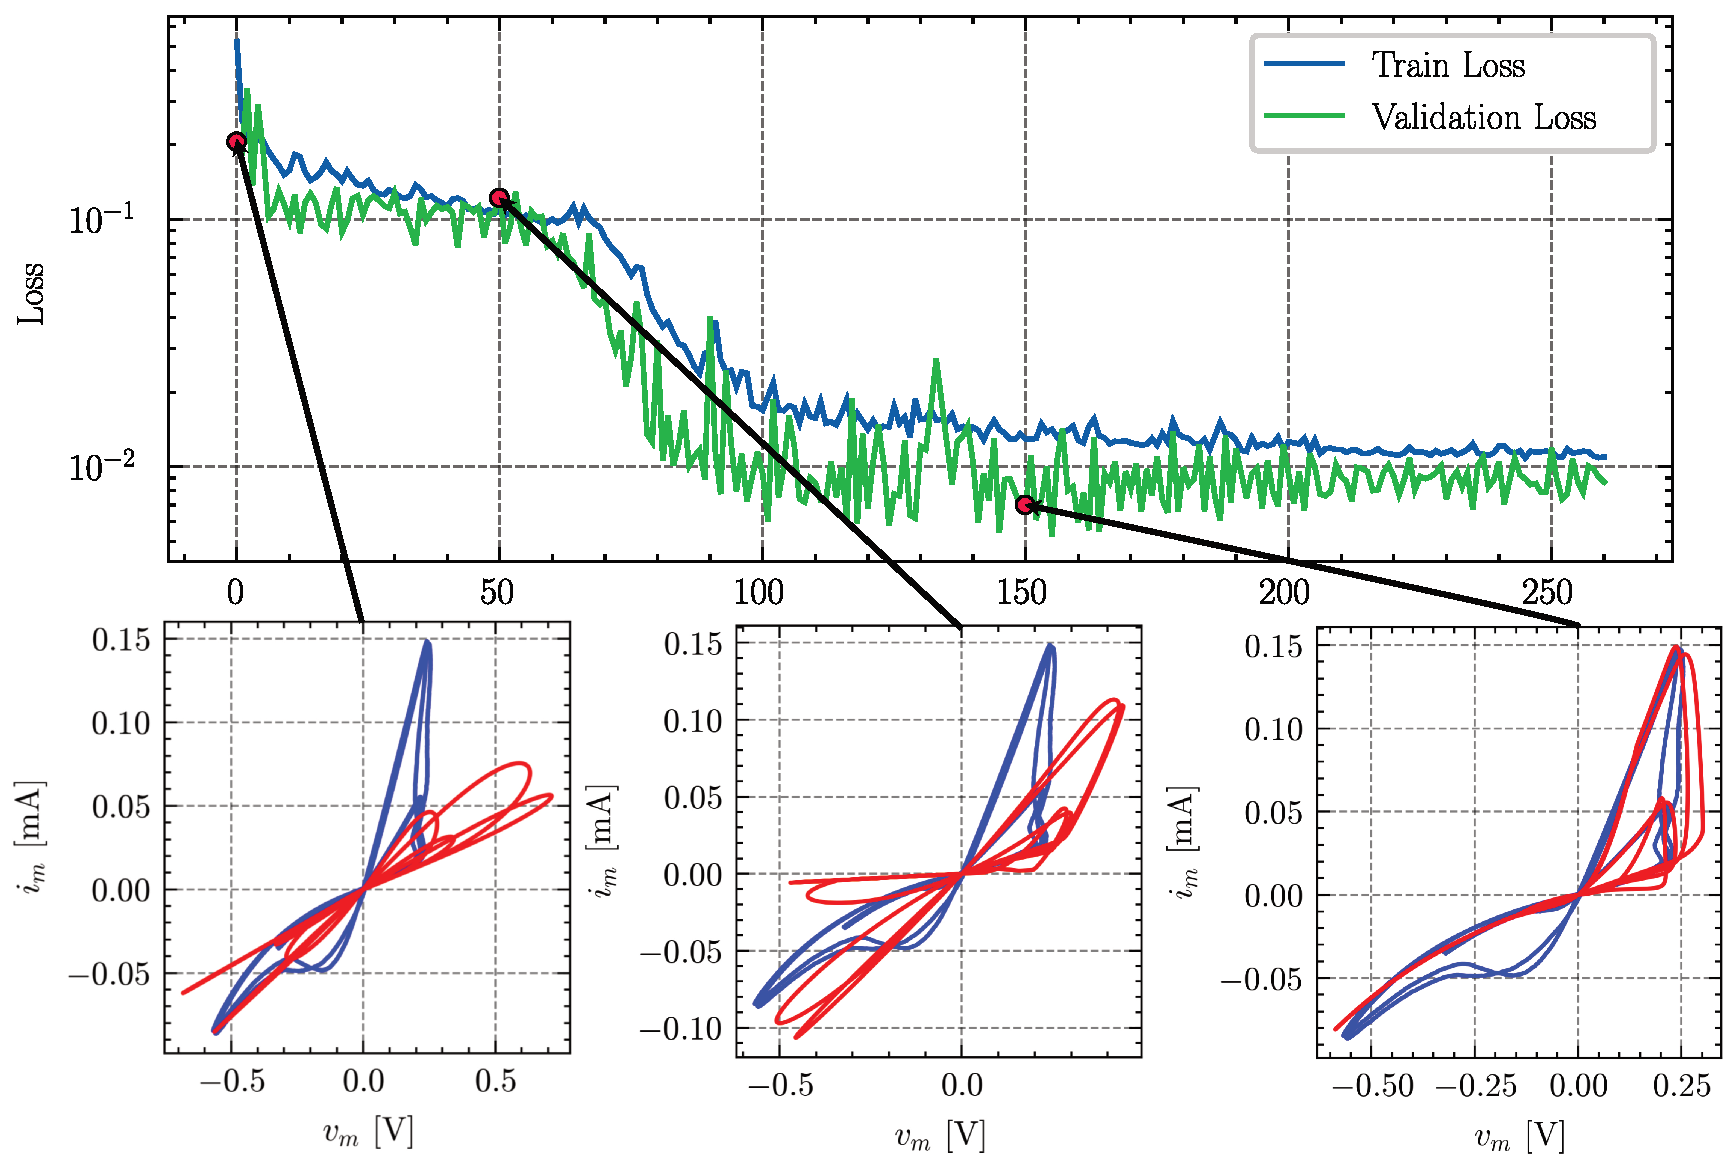
\includegraphics[width=\linewidth]{figs/Training_process.pdf}
  \caption{Learning curve for the Det-MemODE neural network architecture during training over 260 epochs. The plot illustrates the progressive reduction in loss function values for both training and validation datasets, indicating effective optimization and satisfactory model fitting to experimental memristor data. Insets display the evolution of the \(v_m\)--\(i_m\) hysteresis characteristics at selected epochs, demonstrating the model's capability to capture the nonlinear and history-dependent behavior of the memristor as training progresses.}
  \label{fig:learning-curve}
\end{figure}



Representative simulation results demonstrating the neural network model's predictive capabilities are presented in Figure~\ref{fig:sample-results} through comparative analysis of a tungsten-doped memristor device subjected to sinusoidal voltage excitation with an amplitude of 1V and frequency of 1Hz. These specific excitation parameters were selected to capture the characteristic switching dynamics while maintaining operation within the device's linear regime, enabling comprehensive evaluation of the model's ability to reproduce fundamental memristive behaviors.

The analysis encompasses three critical dynamic characteristics that collectively characterize memristor behavior: temporal current evolution, applied voltage profiles, and voltage-current hysteresis relationships. The temporal current response reveals the device's instantaneous electrical behavior and switching kinetics, while the applied voltage profile confirms the fidelity of the input stimulus. Most significantly, the voltage-current hysteresis loops (\(v_m - i_m\)) demonstrate the nonlinear relationship between these electrical quantities and illustrate the fundamental memory properties that define memristive behavior.

The hysteresis loops are particularly diagnostic of memristor performance, as their shape, area, and switching thresholds directly reflect the underlying ionic transport mechanisms and structural modifications responsible for resistive switching. The pinched hysteresis characteristic observed at the origin serves as a definitive signature of memristive behavior, while the loop area quantifies the energy dissipation associated with switching events. These features enable comprehensive validation of the neural network model's ability to capture both the static and dynamic aspects of memristor operation.

\newcommand{\subwidth}{0.48\linewidth}
\begin{figure}[!t]
  \centering
  \subfloat[\label{1a}]{%
    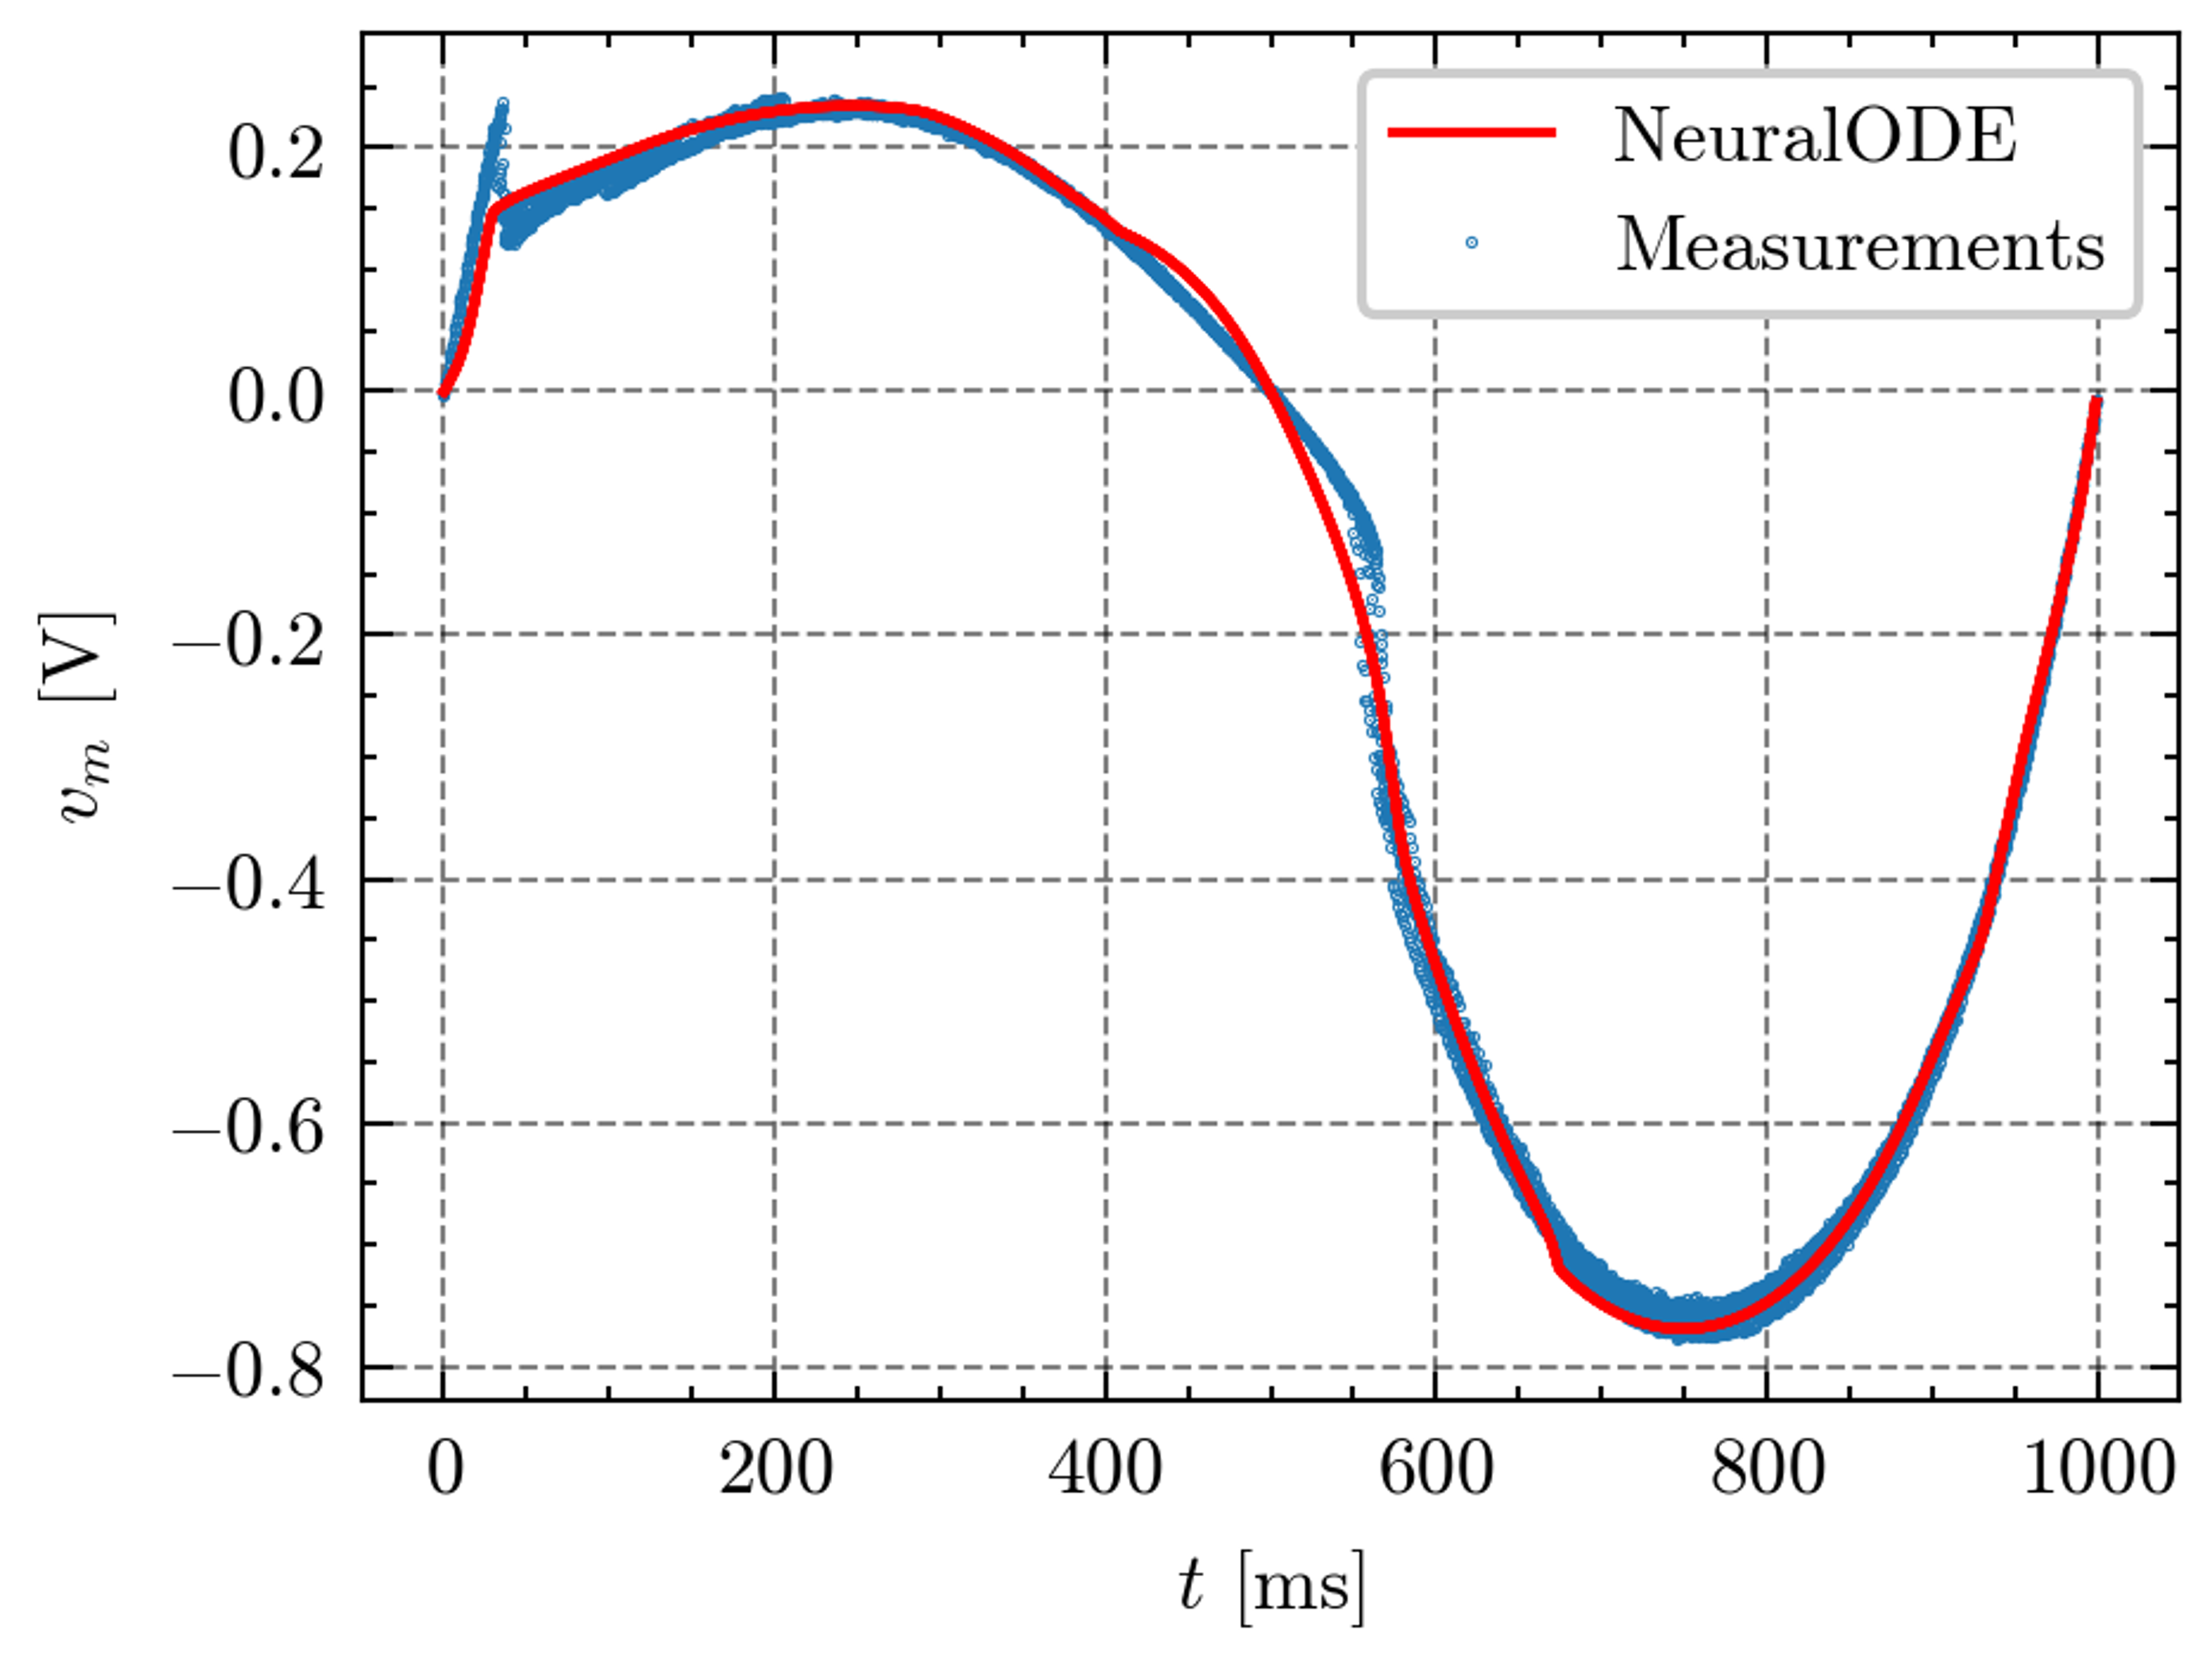
\includegraphics[width=\subwidth]{sample_results/v_m.png}%
  }
  % \hfill
  \subfloat[\label{1b}]{%
    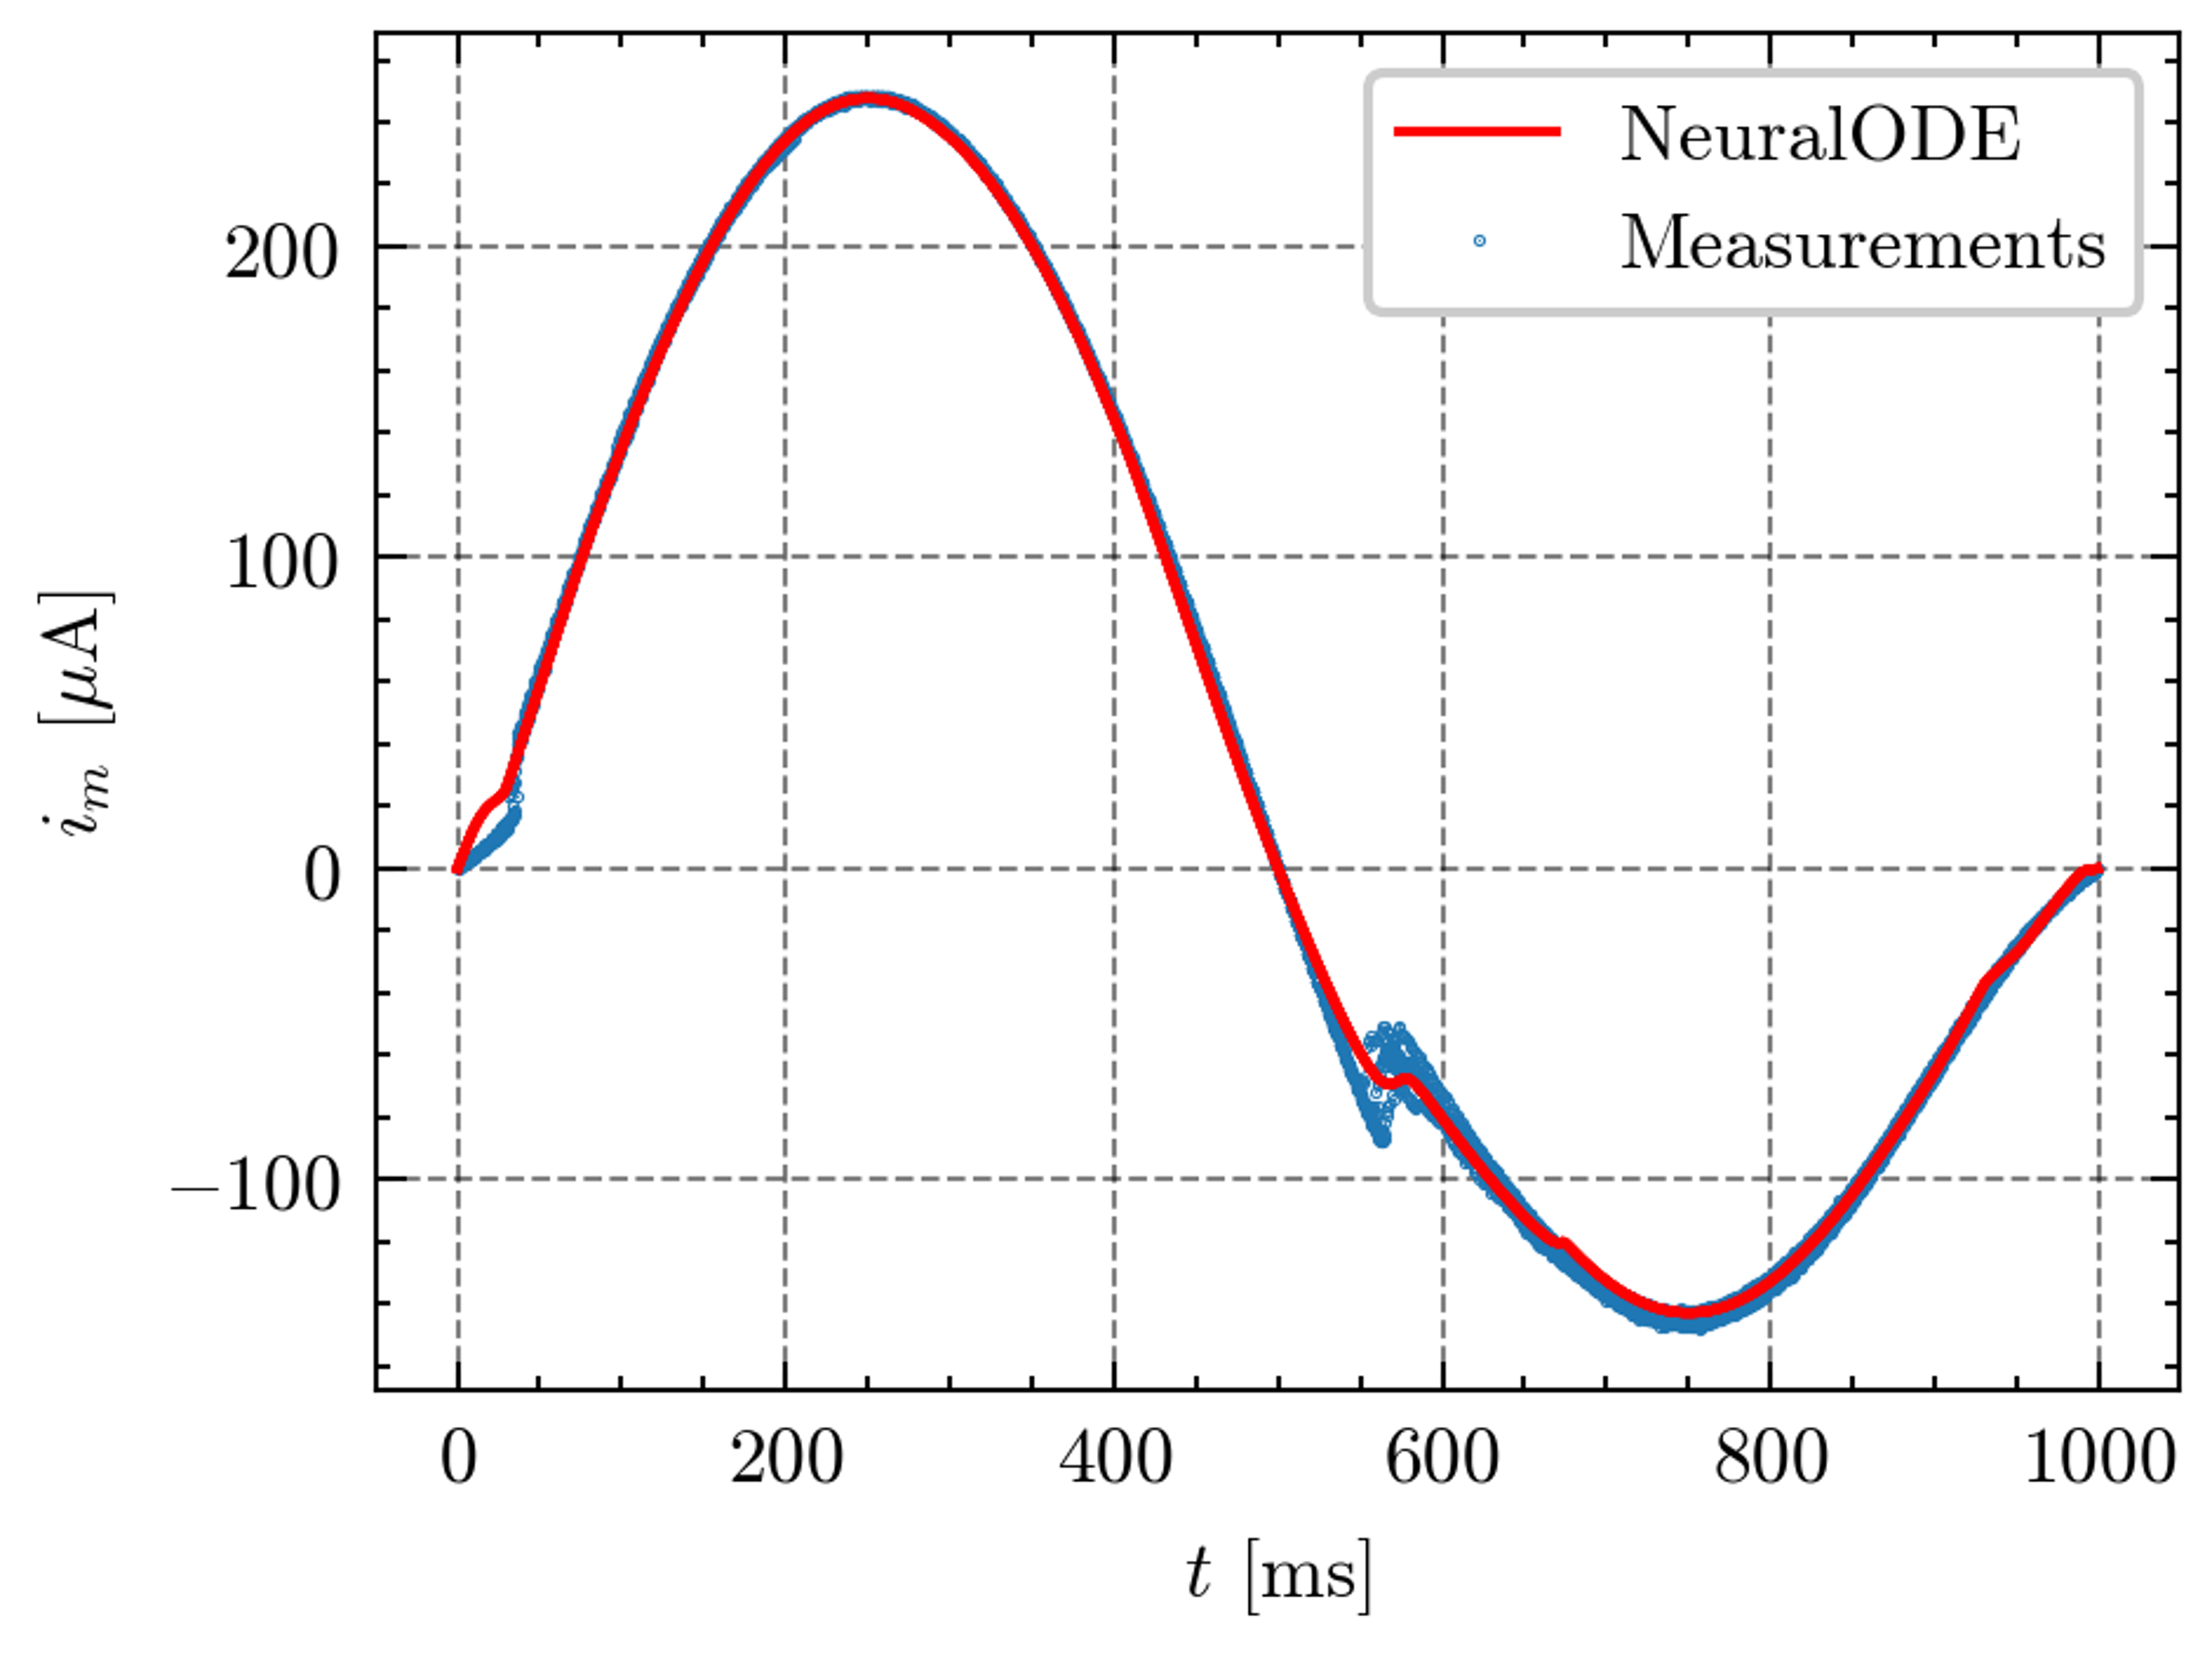
\includegraphics[width=\subwidth]{sample_results/i_m.png}%
  }
  \\
  \subfloat[\label{1c}]{%
    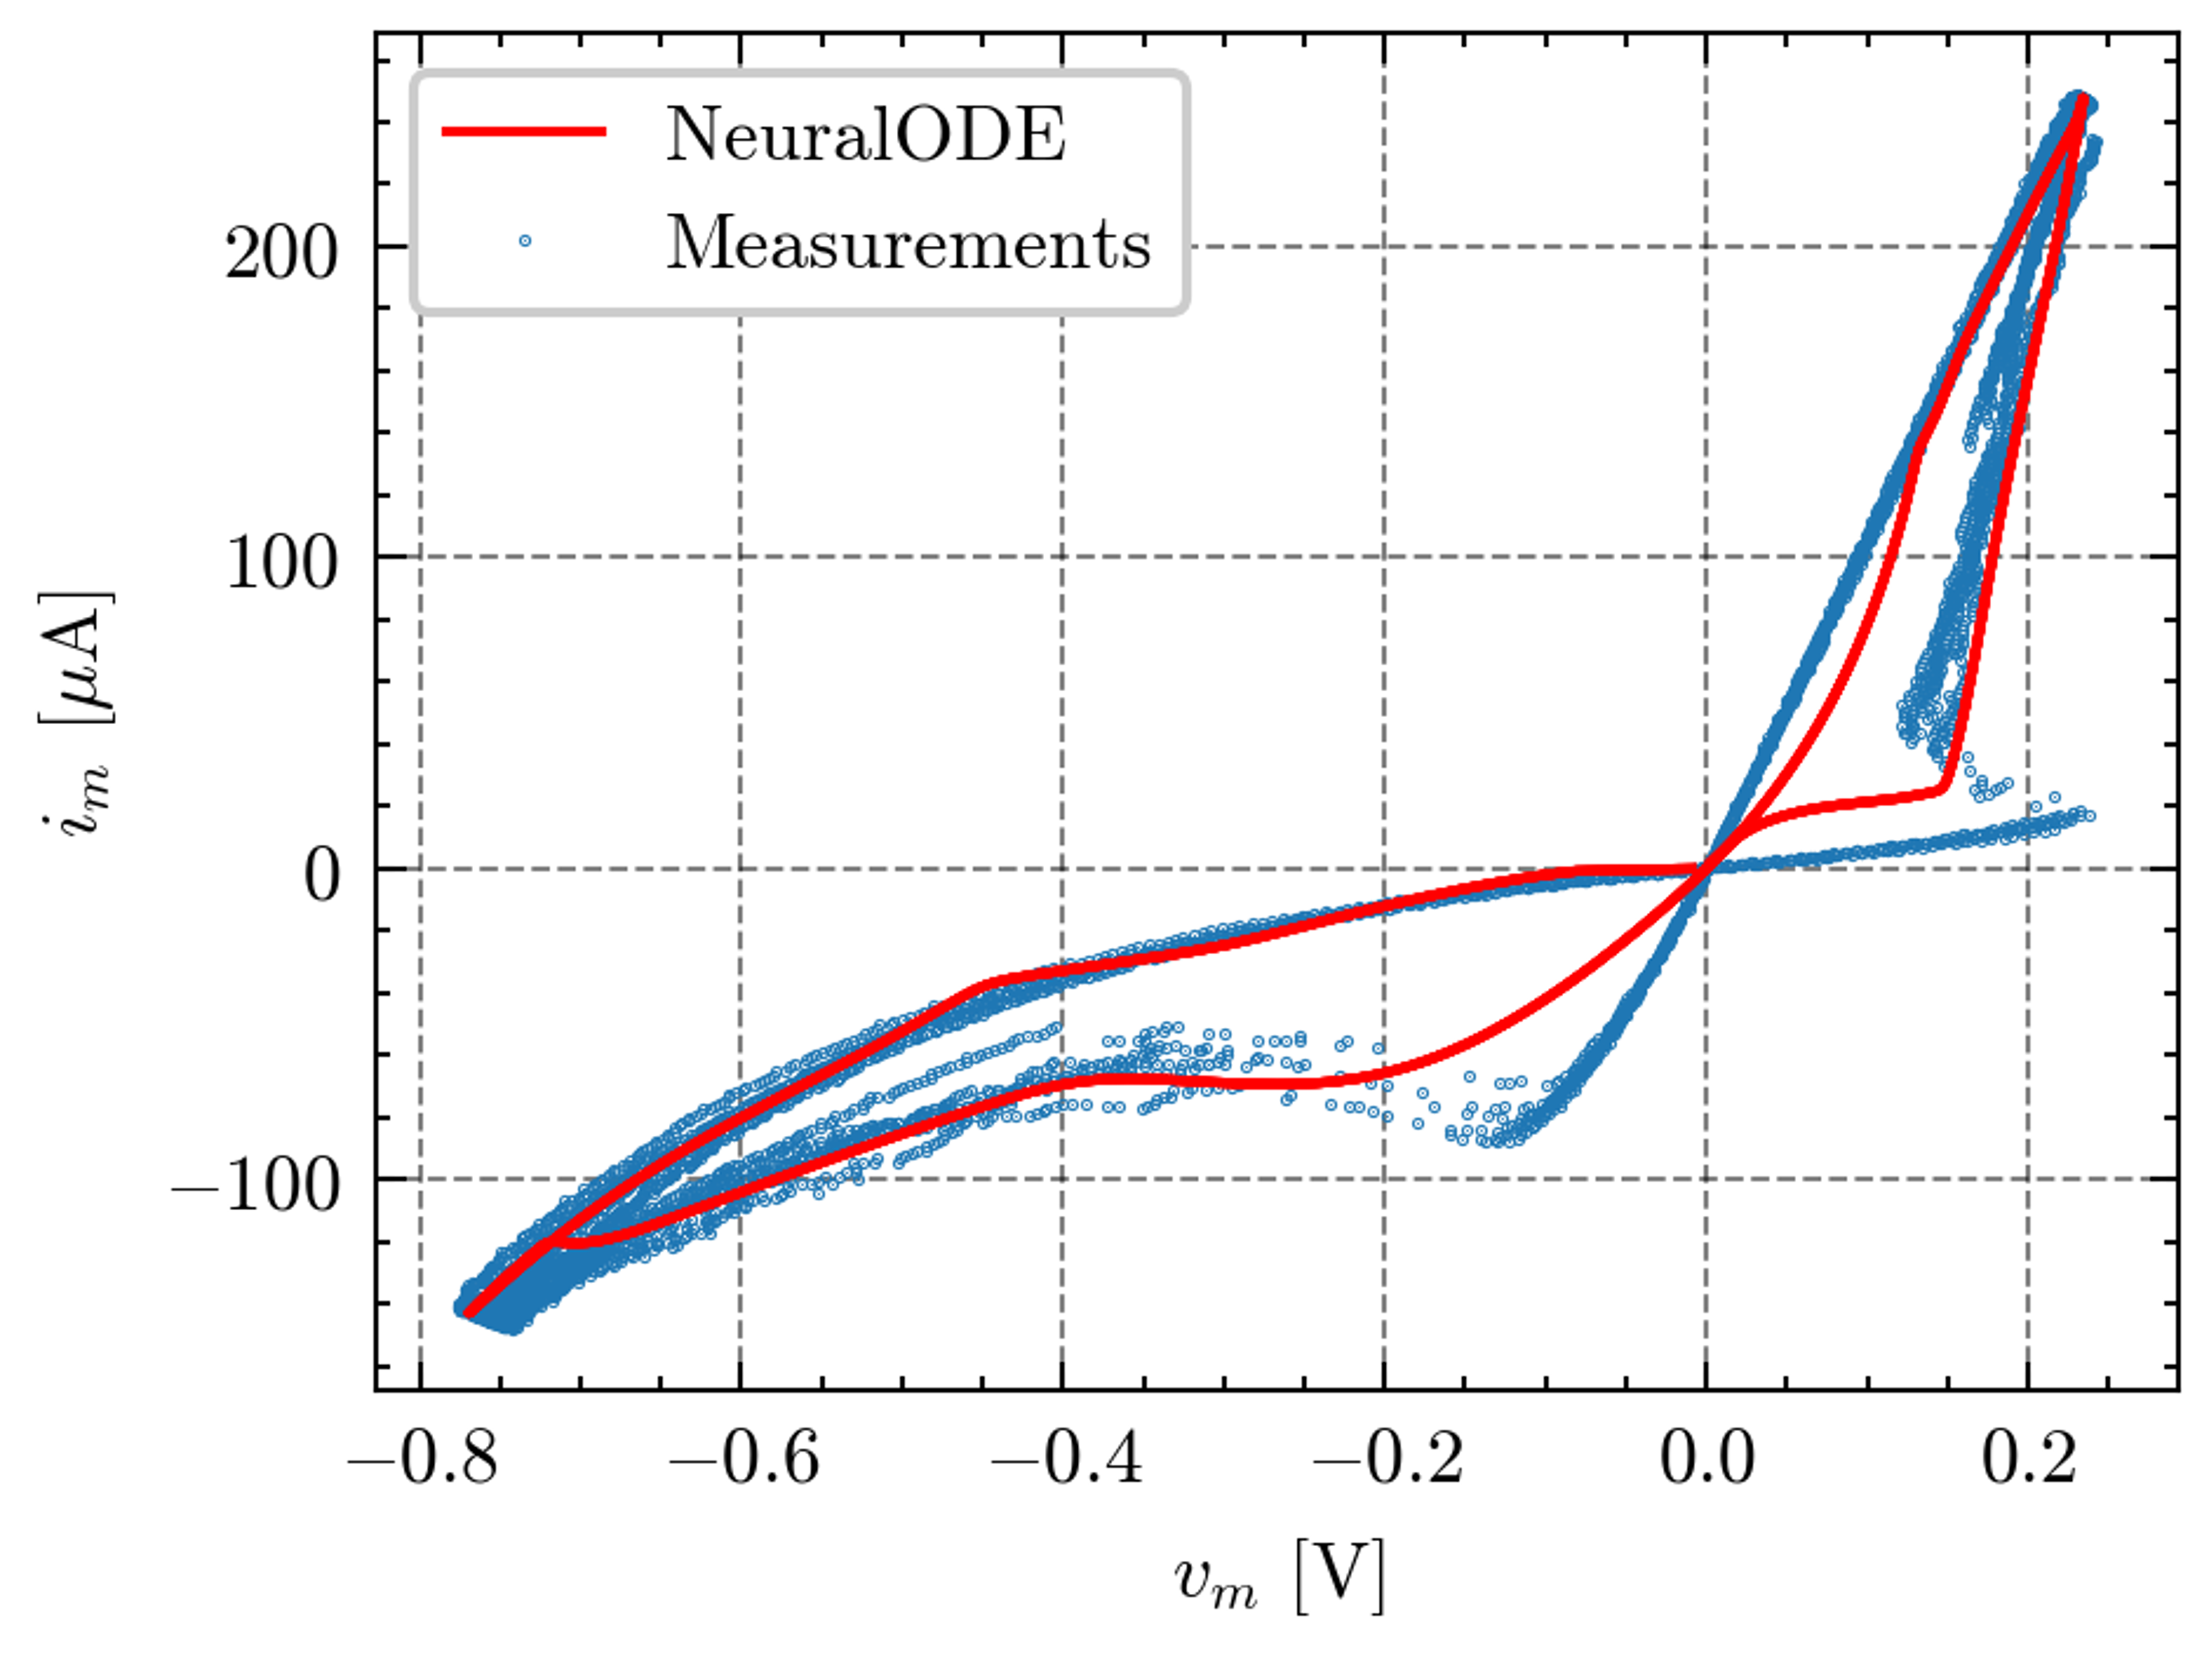
\includegraphics[width=\subwidth]{sample_results/hysteresis.png}%
  }
  \caption{Representative simulation results for tungsten-doped memristor dynamics under sinusoidal voltage excitation (amplitude: 1V, frequency: 1Hz). (a) Applied voltage waveform demonstrating the sinusoidal input stimulus, (b) Predicted memristor current response showing nonlinear temporal evolution and switching characteristics, (c) Voltage-current hysteresis loop (\(v_m - i_m\)) illustrating the characteristic pinched behavior and memory properties fundamental to memristive operation. The neural network model successfully captures the essential features of memristor dynamics including switching thresholds, nonlinear conductance modulation, and hysteretic memory effects. \TODO{Graphs will be replaced}}
  \label{fig:sample-results}
\end{figure}


\subsection{Comparative Analysis with Mean Metastable Switch (MMS) Model and Generalized Mean Metastable Switch (GMMS) Model}

\noindent
To establish the performance advantages of the neural differential equation approach, a comprehensive comparative analysis was conducted between the developed neural network model and the established deterministics model especially conducted for the SDC memristor modelling task: Mean Metastable Switch (MMS) with the Eq. \eqref{eq:mms} and Generalized Mean Metastable Switch (GMMS) model with the Eq. \eqref{eq:gmms}.

This comparison is particularly significant as the MMS model has been extensively validated against experimental data and serves as a benchmark for memristor circuit simulation in the scientific literature. The comparative evaluation encompasses temporal voltage and current evolution, hysteretic characteristics, and quantitative loss function metrics to provide comprehensive assessment of modeling fidelity across multiple performance dimensions.

Quantitative analysis reveals substantial performance improvements achieved by the neural network approach. The average loss function value for the Det-MemODE neural network model was \(0.015223\), and \(0.002226\) for the Dual-NN-MemODE model, representing a significant improvement compared to the MMS model's average loss of \(0.072356\), and GMMS model \(0.035835\). This near two times reduction in loss indicates markedly superior agreement between neural network predictions and experimental data, demonstrating the enhanced modeling capability achieved through the neural differential equation framework.


The superior performance of the neural network model can be attributed to its capacity for learning complex nonlinear mappings directly from experimental data, whereas the MMS model relies on predetermined phenomenological relationships that may not fully capture the device-specific dynamics and material-dependent switching characteristics inherent in experimental memristor devices.
\newcommand{\redbar}{\protect\tikz[baseline=-0.1ex]\fill[ieeered] (0,0) rectangle (0.8em,1.2ex);}\newcommand{\bluebar}{\protect\tikz[baseline=-0.1ex]\fill[ieeeblue] (0,0) rectangle (0.8em,1.2ex);}
\newcommand{\greenbar}{\protect\tikz[baseline=-0.1ex]\fill[ieeegreen] (0,0) rectangle (0.8em,1.2ex);}

\begin{figure*}[!t]
  \centering
  \subfloat[\label{1a}]{%
    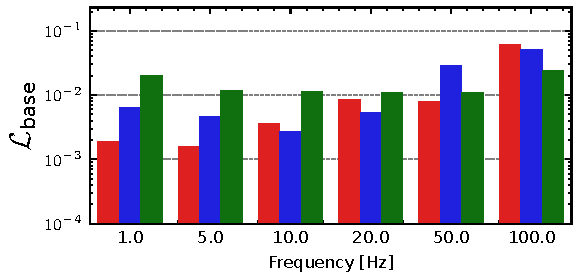
\includegraphics[width=0.48\linewidth]{mms_results/loss_per_freq_Det-MemODE.pdf}%
  }
  \subfloat[\label{1b}]{%
    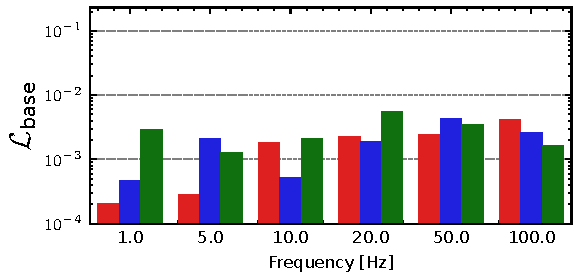
\includegraphics[width=0.48\linewidth]{mms_results/loss_per_freq_Dual-NN-MemODE.pdf}%
  }

  \subfloat[\label{1c}]{%
    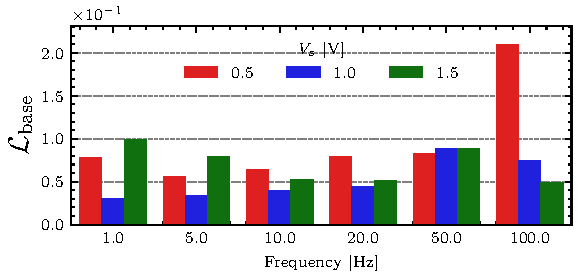
\includegraphics[width=0.48\linewidth]{mms_results/loss_per_freq_MMS Model.pdf}%
  }
  \subfloat[\label{1d}]{%
    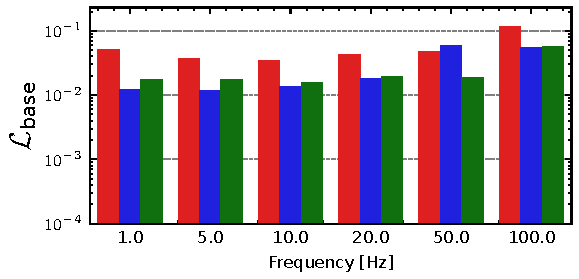
\includegraphics[width=0.48\linewidth]{mms_results/loss_per_freq_GMMS Model.pdf}%
  }
  \caption{Comparative analysis of loss function evolution where the following colors distinguish different supply voltage amplitudes: (\redbar{})~\(V_s=0.5\rm \ V\), (\bluebar{})~\(V_s=1.0\rm \ V\), and (\greenbar{}) \(V_s=1.5\rm \ V\). The models compared are (a) the Det-MemODE model, (b) the Dual-NN-MemODE model, (c) the Mean Mean Metastable Switch (MMS) model, and (d) the Generalized Mean Metastable Switch (GMMS) model. The neural network demonstrates superior convergence characteristics and achieves significantly lower final loss values, indicating enhanced modeling accuracy and better agreement with experimental memristor dynamics.}
  \label{fig:comparison_mms}
\end{figure*}

Table~\ref{tab:mms_comp} presents a comparative analysis of the representative loss functions obtained for the neural network and MMS models, offering a quantitative assessment of their performance across key electrical characteristics. The results highlight the neural network’s enhanced capability to reproduce complex and subtle aspects of memristor dynamics that are insufficiently captured by the phenomenological MMS/GMMS framework. For clarity, the highest loss value in each row is marked in red, whereas the lowest is marked in green. Overall, the neural network model consistently achieves substantially lower loss values, demonstrating superior accuracy and fidelity in representing the device behavior.

\begin{table}
  \caption{Comparative \(\mathcal{L}_{\mathrm{base}}\) loss function analysis.}
  \label{tab:mms_comp}
  \centering
  \begin{tabular}{c|cccc}
    \toprule
    \multicolumn{5}{c}{\textbf{Loss function comparison for \(V_s = 0.5 \rm \ V\)}}                                                                                        \\
    \midrule
    \(f_s\) [Hz] & \makecell{Det-                                                                                                                                          \\MemODE}             & \makecell{Dual-NN-                                                                                                             \\ MemODE}                 & \makecell{GMMS\\Model}             & \makecell{MMS\\Model}                                        \\
    \midrule
    \textbf{1}   & \(1.92 \cdot 10^{-3}\) & \color{ieeegreen} \bfseries \(2.07 \cdot 10^{-4}\) & \(5.21 \cdot 10^{-2}\) & \color{ieeered} \bfseries \(7.86 \cdot 10^{-2}\) \\
    \textbf{5}   & \(1.60 \cdot 10^{-3}\) & \color{ieeegreen} \bfseries \(2.85 \cdot 10^{-4}\) & \(3.70 \cdot 10^{-2}\) & \color{ieeered} \bfseries \(5.59 \cdot 10^{-2}\) \\
    \textbf{10}  & \(3.64 \cdot 10^{-3}\) & \color{ieeegreen} \bfseries \(1.83 \cdot 10^{-3}\) & \(3.43 \cdot 10^{-2}\) & \color{ieeered} \bfseries \(6.44 \cdot 10^{-2}\) \\
    \textbf{20}  & \(8.69 \cdot 10^{-3}\) & \color{ieeegreen} \bfseries \(2.27 \cdot 10^{-3}\) & \(4.24 \cdot 10^{-2}\) & \color{ieeered} \bfseries \(7.96 \cdot 10^{-2}\) \\
    \textbf{50}  & \(7.86 \cdot 10^{-3}\) & \color{ieeegreen} \bfseries \(2.47 \cdot 10^{-3}\) & \(4.71 \cdot 10^{-2}\) & \color{ieeered} \bfseries \(8.29 \cdot 10^{-2}\) \\
    \textbf{100} & \(6.24 \cdot 10^{-2}\) & \color{ieeegreen} \bfseries \(4.21 \cdot 10^{-3}\) & \(1.18 \cdot 10^{-1}\) & \color{ieeered} \bfseries \(2.10 \cdot 10^{-1}\) \\
    \bottomrule
  \end{tabular}
  \begin{tabular}{c|cccc}
    \toprule
    \multicolumn{5}{c}{\textbf{Loss function comparison for \(V_s = 1 \rm \ V\)}}                                                                                          \\
    \midrule
    \(f_s\) [Hz] & \makecell{Det-                                                                                                                                          \\MemODE}             & \makecell{Dual-NN-                                                                                                             \\ MemODE}                 & \makecell{GMMS\\Model}             & \makecell{MMS\\Model}                                        \\
    \midrule
    \textbf{1}   & \(6.40 \cdot 10^{-3}\) & \color{ieeegreen} \bfseries \(4.69 \cdot 10^{-4}\) & \(1.20 \cdot 10^{-2}\) & \color{ieeered} \bfseries \(3.08 \cdot 10^{-2}\) \\
    \textbf{5}   & \(4.58 \cdot 10^{-3}\) & \color{ieeegreen} \bfseries \(2.11 \cdot 10^{-3}\) & \(1.19 \cdot 10^{-2}\) & \color{ieeered} \bfseries \(3.37 \cdot 10^{-2}\) \\
    \textbf{10}  & \(2.74 \cdot 10^{-3}\) & \color{ieeegreen} \bfseries \(5.27 \cdot 10^{-4}\) & \(1.36 \cdot 10^{-2}\) & \color{ieeered} \bfseries \(3.93 \cdot 10^{-2}\) \\
    \textbf{20}  & \(5.32 \cdot 10^{-3}\) & \color{ieeegreen} \bfseries \(1.90 \cdot 10^{-3}\) & \(1.84 \cdot 10^{-2}\) & \color{ieeered} \bfseries \(4.43 \cdot 10^{-2}\) \\
    \textbf{50}  & \(2.88 \cdot 10^{-2}\) & \color{ieeegreen} \bfseries \(4.26 \cdot 10^{-3}\) & \(5.86 \cdot 10^{-2}\) & \color{ieeered} \bfseries \(8.91 \cdot 10^{-2}\) \\
    \textbf{100} & \(5.08 \cdot 10^{-2}\) & \color{ieeegreen} \bfseries \(2.63 \cdot 10^{-3}\) & \(5.45 \cdot 10^{-2}\) & \color{ieeered} \bfseries \(7.45 \cdot 10^{-2}\) \\
    \bottomrule
  \end{tabular}
  \begin{tabular}{c|cccc}
    \toprule
    \multicolumn{5}{c}{\textbf{Loss function comparison for \(V_s = 1.5 \rm \ V\)}}                                                                                                                  \\
    \midrule
    \(f_s\) [Hz] & \makecell{Det-                                                                                                                                                                    \\MemODE}             & \makecell{Dual-NN-                                                                                                             \\ MemODE}                 & \makecell{GMMS\\Model}             & \makecell{MMS\\Model}                                        \\
    \midrule
    \textbf{1}   & \(1.99 \cdot 10^{-2}\) & \color{ieeegreen} \bfseries \(2.95 \cdot 10^{-3}\) & \(1.77 \cdot 10^{-2}\)                           & \color{ieeered} \bfseries \(9.95 \cdot 10^{-2}\) \\
    \textbf{5}   & \(1.17 \cdot 10^{-2}\) & \color{ieeegreen} \bfseries \(1.26 \cdot 10^{-3}\) & \(1.73 \cdot 10^{-2}\)                           & \color{ieeered} \bfseries \(7.88 \cdot 10^{-2}\) \\
    \textbf{10}  & \(1.14 \cdot 10^{-2}\) & \color{ieeegreen} \bfseries \(2.08 \cdot 10^{-3}\) & \(1.56 \cdot 10^{-2}\)                           & \color{ieeered} \bfseries \(5.24 \cdot 10^{-2}\) \\
    \textbf{20}  & \(1.09 \cdot 10^{-2}\) & \color{ieeegreen} \bfseries \(5.51 \cdot 10^{-3}\) & \(1.96 \cdot 10^{-2}\)                           & \color{ieeered} \bfseries \(5.09 \cdot 10^{-2}\) \\
    \textbf{50}  & \(1.09 \cdot 10^{-2}\) & \color{ieeegreen} \bfseries \(3.46 \cdot 10^{-3}\) & \(1.87 \cdot 10^{-2}\)                           & \color{ieeered} \bfseries \(8.90 \cdot 10^{-2}\) \\
    \textbf{100} & \(2.44 \cdot 10^{-2}\) & \color{ieeegreen} \(1.65 \cdot 10^{-3}\)           & \color{ieeered} \bfseries \(5.63 \cdot 10^{-2}\) & \(4.87 \cdot 10^{-2}\)                           \\
    \bottomrule
  \end{tabular}
\end{table}


\subsection{Hyperparameter Sensitivity Analysis}
\noindent Hyperparameter optimization was conducted to systematically explore the parameter space and identify configurations that maximize the predictive performance of the neural network. The optimization employed the Tree-structured Parzen Estimator (TPE) algorithm, implemented in the \verb|Optuna| framework~\cite{akiba2019optuna}. The TPE algorithm models the objective function probabilistically by constructing two separate density estimators: one for configurations associated with above-average performance and another for those yielding below-average results. By sampling preferentially from the former, while still maintaining diversity through exploration of the latter, the algorithm achieves an efficient balance between exploitation of promising regions and exploration of the broader search space.

The search space encompassed both architectural and training-related hyperparameters. On the architectural side, the number of hidden layers was varied between one and five, with layer widths ranging from 16 to 512 neurons in increments of 16. Candidate activation functions included widely used nonlinearities such as ReLU, GELU, SiLU, \(\tanh\), ELU, leaky ReLU, and sigmoid, as well as identity and sine functions. For the output layer, the choice was restricted to \({\text{linear}, \tanh, \text{sigmoid}, \text{ReLU}}\). The training-related search space included the learning rate, sampled on a logarithmic scale between \(10^{-4}\) and \(10^{-1}\), batch size ranging from 1 to 18, optimizer type (Adam, SGD, AdamW, Nadam, AdaBelief), and additional parameters related to regularization and scheduling, including patience, cooldown, reduction factor, tolerance, and weight decay.

To quantify the relative influence of individual hyperparameters on model performance, a surrogate-based importance analysis was performed. An XGBoost gradient boosting model~\cite{Chen2016} was trained on the explored configurations to predict validation loss. The surrogate achieved an \(\mathrm{R}^2\) value of 0.99, indicating high fidelity in capturing the dependence of model performance on hyperparameter selection. Importance was first estimated using the \emph{gain} metric, which reflects the cumulative improvement in predictive accuracy attributable to each hyperparameter across the ensemble. Normalization ensured that scores summed to unity, allowing for direct interpretation as relative contributions to performance variability.

As a complementary approach, permutation importance~\cite{Altmann2010} was applied to the surrogate model. In this procedure, the values of each hyperparameter were permuted at random, and the resulting degradation in predictive accuracy was recorded. Repeated ten times for each feature, the mean error increase provided an alternative measure of importance, which, unlike gain-based metrics, also accounts for nonlinear dependencies and interactions among hyperparameters.

Both approaches consistently identified the learning rate and gradient clipping value as the dominant hyperparameters. According to the gain-based measure, their contributions were 0.10 and 0.74, respectively, while the permutation-based analysis yielded corresponding values of 0.44 and 0.30. Together, these two parameters explained approximately 63\% of the observed variance in performance. By contrast, the activation function exhibited only marginal influence (importance score of 0.04), indicating that the Neural ODE architecture is relatively robust to this choice within the tested range.

\begin{figure}[!t]
  \centering
  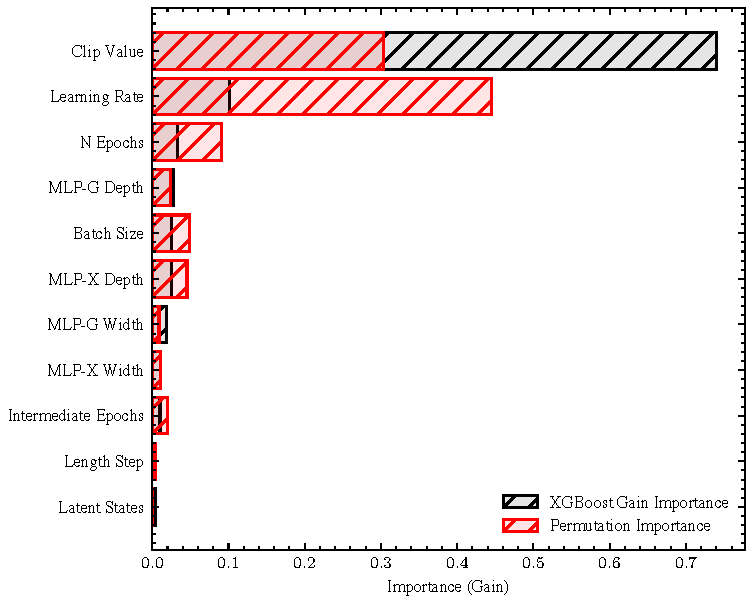
\includegraphics[width=\linewidth]{mms_figs/xgboost_permutation_importance.pdf}
  \caption{Hyperparameter importance for the Dual-NN-MemODE optimization task. Scores were computed using permutation importance applied to an XGBoost surrogate model trained on 200 hyperparameter configurations. Larger values indicate greater relative influence of the corresponding hyperparameter on model performance.}
  \label{fig:hyperparameter_importance}
\end{figure}






\printbibliography

\begin{IEEEbiographynophoto}{Jane Doe}
  Biography text here without a photo.
\end{IEEEbiographynophoto}

\begin{IEEEbiography}[{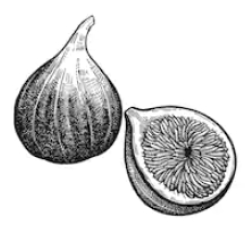
\includegraphics[width=1in,height=1.25in,clip,keepaspectratio]{fig1.png}}]{IEEE Publications Technology Team}
  In this paragraph you can place your educational, professional background and research and other interests.\end{IEEEbiography}


\end{document}


